% Metódy inžinierskej práce

\documentclass[10pt,twoside,slovak,a4paper]{article}

\usepackage[slovak]{babel}
%\usepackage[T1]{fontenc}
\usepackage[IL2]{fontenc} % lepšia sadzba písmena Ľ než v T1
\usepackage[utf8]{inputenc}
\usepackage{graphicx}
\usepackage{url} % príkaz \url na formátovanie URL
\usepackage{hyperref} % odkazy v texte budú aktívne (pri niektorých triedach dokumentov spôsobuje posun textu)

\usepackage{cite}
%\usepackage{times}

\pagestyle{headings}

\title{Vplývajú mobilné technológie na študentov vo výučbe predmetu matematika?\thanks{Semestrálny projekt v predmete Metódy inžinierskej práce, ak. rok 2020/21, vedenie: Ing. Jozef Sitarčík}} % meno a priezvisko vyučujúceho na cvičeniach

\author{Tamara Janotková\\[2pt]
	{\small Slovenská technická univerzita v Bratislave}\\
	{\small Fakulta informatiky a informačných technológií}\\
	{\small \texttt{xjanotkovat@stuba.sk}}
	}

\date{\small 15. október 2020} % upravte



\begin{document}

\maketitle

\begin{abstract}
V dnešnej dobe vysokého technologického pokroku, ktorý sa vyvíja obrovským tempom, by sme sotva hľadali odvetvie, v ktorom mobilné technológie nemajú využitie. Zamerajúc sa na prostredie vzdelávania ide hlavne o integrovanie mobilných zariadení či tabletov do procesu výučby. V širšom ponímaní, naša práca je zameraná na tému vzdelávania pomocou technológií. Presnejšie sa jedná o využitie mobilných technológií vo výučbe predmetu matematika. Už spomínané mobilné zariadenia, dokážu v edukačnom procese nielen nahradiť učebnice, no najmä zefektívniť výučbu, či už pomocou množstva softvérov, ktoré umožnia lepšie pochopenie danej témy, ale i uľahčenie komunikácie medzi študentom a učiteľom alebo študentami navzájom. Z nášho pohľadu je priam na mieste otázka, ktorej sa v článku chceme venovať: ako, a či vôbec dokážu technológie ovplyvniť študijné výsledky študentov a ich osobný postoj k matematike, počas ktorej spomínané technológie využívajú. 
\end{abstract}



\section{Úvod}

Mobilné technológie a mladí ľudia sú od nepamäti považovaní za veľmi blízkych spoločníkov. V obrovskej množine mladých sa vyskytuje len málo jedincov, ktorí s použitím mobilných technológií nemajú skúsenosti. Vo väčšine prípadov mladý človek na používanie mobilných technológií reaguje pozitívne, ba čo viac, považuje ich za akýsi kľúč ku ľahšiemu životu. Naopak, to, čo robí život mladého človeka v jeho očiach ťažkým je mnohokrát štúdium. Idúc do hĺbky, kameňom úrazu býva práve odvetvie matematiky. Nasledujúce kapitoly nám poskytnú pohľad na kombináciu príjemného s užitočným- kombináciu matematiky a mobilných technológií vo výučbovom procese. V ~\ref{nejaka} kapitole si objasníme čo spomínané mobilné technológie sú, aké konkrétne využitie majú v procese výučby a predstavíme si zopár matematických softvérov. ~\ref{ina} kapitola je venovaná problematike efektívneho učenia.~\ref{dolezita} kapitola sa zameriava na konkrétne použitie mobilných technológií vo výučbe matematiky. Výsledky sú zhrnuté v záverečnej časti.

\section{Mobilné technológie} \label{nejaka}

tu def MT 

\subsection{Využitie mobilných technológií} \label{ina:vyuzitie}

nejake...

\subsection{Matematické softvéry} \label{ina:softvery}

Z obr.~\ref{f:rozhod} je všetko jasné. 

\begin{figure*}[tbh]
\centering
%\includegraphics[scale=1.0]{diagram.pdf}
Aj text môže byť prezentovaný ako obrázok. Stane sa z neho označný plávajúci objekt. Po vytvorení diagramu zrušte znak \texttt{\%} pred príkazom \verb|\includegraphics| označte tento riadok ako komentár (tiež pomocou znaku \texttt{\%}).

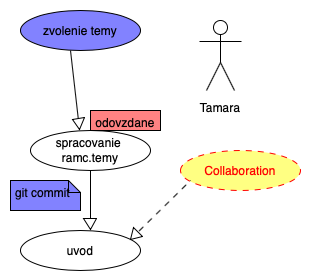
\includegraphics[scale=0.5]{prvy.png}
\caption{Rozhodujúci argument.}
\label{f:rozhod}
\end{figure*}



\section{Efektívne učenie} \label{ucenie}

Základným problémom je teda\ldots{} Najprv sa pozrieme na nejaké vysvetlenie (časť~\ref{ina:nejake}), a potom na ešte nejaké (časť~\ref{ina:nejake}).\footnote{Niekedy môžete potrebovať aj poznámku pod čiarou.}

Môže sa zdať, že problém vlastne nejestvuje\cite{Coplien:MPD}, ale bolo dokázané, že to tak nie je~\cite{Czarnecki:Staged, Czarnecki:Progress}. Napriek tomu, aj dnes na webe narazíme na všelijaké pochybné názory\cite{PLP-Framework}. Dôležité veci možno \emph{zdôrazniť kurzívou}.


Niekedy treba uviesť zoznam:

\begin{itemize}
\item jedna vec
\item druhá vec
	\begin{itemize}
	\item x
	\item y
	\end{itemize}
\end{itemize}

Ten istý zoznam, len číslovaný:

\begin{enumerate}
\item jedna vec
\item druhá vec
	\begin{enumerate}
	\item x
	\item y
	\end{enumerate}
\end{enumerate}


\paragraph{Veľmi dôležitá poznámka.}
Niekedy je potrebné nadpisom označiť odsek. Text pokračuje hneď za nadpisom.



\section{Matematika a mobilné technológie} \label{dolezita}


\section{Záver} \label{zaver} % prípadne iný variant názvu



%\acknowledgement{Ak niekomu chcete poďakovať\ldots}


% týmto sa generuje zoznam literatúry z obsahu súboru literatura.bib podľa toho, na čo sa v článku odkazujete
\bibliography{literatura}
\bibliographystyle{plain} % prípadne alpha, abbrv alebo hociktorý iný
\end{document}
